\documentclass[12pt, a4paper]{article}

\usepackage[utf8]{inputenc}
\usepackage[T1]{fontenc}
\usepackage[brazilian]{babel}
\usepackage{mathptmx}
\usepackage{amsmath, amssymb}
\usepackage{graphicx}
\usepackage{booktabs}
\usepackage{geometry}
\usepackage{float}
\usepackage{setspace}
\usepackage{caption}

\geometry{top=3cm, bottom=2cm, left=3cm, right=2cm}
\setstretch{1.5}
\captionsetup{font=small, labelfont=bf, labelsep=endash}

\begin{document}

\begin{center}
    \Large\textbf{Relatório Intermediário de Benchmarking -- Cenário 5} \\[0.2cm]
    \large\textit{A Sinergia do DataOps: Otimização de Hardware e o Efeito ``Too Fast to Cache''} \\[0.5cm]
    \normalsize\textbf{Projeto DataOps / UNIFEI} \\
    \small{\today}
\end{center}

\vspace{0.5cm}
\noindent\rule{\textwidth}{1pt}

\section*{1. Descrição do Cenário e Progressão Histórica}
O Cenário 4 comprovou que a compactação de dados estruturais era a chave para mitigar o gargalo de I/O do Apache Druid, estabilizando as respostas na escala de milissegundos mesmo com recursos limitados (2 núcleos). Neste \textbf{Cenário 5}, a pesquisa avança aplicando a escalabilidade vertical adequada: dobrou-se o poder computacional para \textbf{4 núcleos de processamento}, operando sobre a mesma base compactada anualmente (\textit{CompactYear}).

\section*{2. Análise Sequencial: O Impacto Real do Paralelismo}
A Tabela 1 revela que o paralelismo, quando executado sobre uma base sem fragmentação extrema, entrega benefícios diretos em cargas analíticas intensas.

\begin{table}[H]
\centering
\caption{Resultados do Cenário 5 - Dados Compactados com 4 Núcleos}
\vspace{0.2cm}
\begin{tabular}{@{}lcccc@{}}
\toprule
\textbf{Domínio da Consulta SQL} & \textbf{Cold (ms)} & \textbf{Warm (ms)} & \textbf{Otimização} & \textbf{Registros} \\
\midrule
    Bench 1 Serie Temporal & 48.69 & 27.98 & 42.54\% & 100 \\
    Bench 2 Alta Cardinalidade & 119.29 & 43.63 & 63.43\% & 50 \\
    Bench 3 Filtros Complexos & 27.93 & 28.80 & -3.14\% & 9 \\
    BI 1 ONS Infraestrutura & 65.33 & 39.23 & 39.95\% & 15 \\
    BI 2 FUNAI Terras Indigenas & 46.41 & 29.73 & 35.93\% & 10 \\
    BI 3 Defesa Civil Risco & 96.26 & 23.38 & 75.71\% & 81 \\

\bottomrule
\end{tabular}
\end{table}

\subsection*{2.1. O Brilho da Alta Cardinalidade}
A evidência mais contundente da eficácia computacional ocorreu na consulta \textit{Bench\_2\_Alta\_Cardinalidade}. No Cenário 4 (2 núcleos), esta operação exigia \textbf{461.91 ms} em \textit{Cold Start}. Ao alocar 4 núcleos, a mesma operação foi resolvida em impressionantes \textbf{119.29 ms}. O ganho é matemático: o nó \textit{Historical} agora possui \textit{threads} adicionais para processar agrupamentos (GROUP BY) em paralelo sobre os segmentos compactos em memória mapeada (\textit{mmap}).

\subsection*{2.2. O Fenômeno ``Too Fast to Cache''}
Um comportamento fascinante foi documentado na consulta \textit{Bench\_3\_Filtros\_Complexos}. A latência de leitura direta (Cold) marcou incriveis \textbf{27.93 ms}, enquanto a leitura do Cache (Warm) marcou \textbf{28.80 ms}, gerando um ganho negativo aparente de \textbf{-3.14\%}.

\begin{figure}[H]
\centering
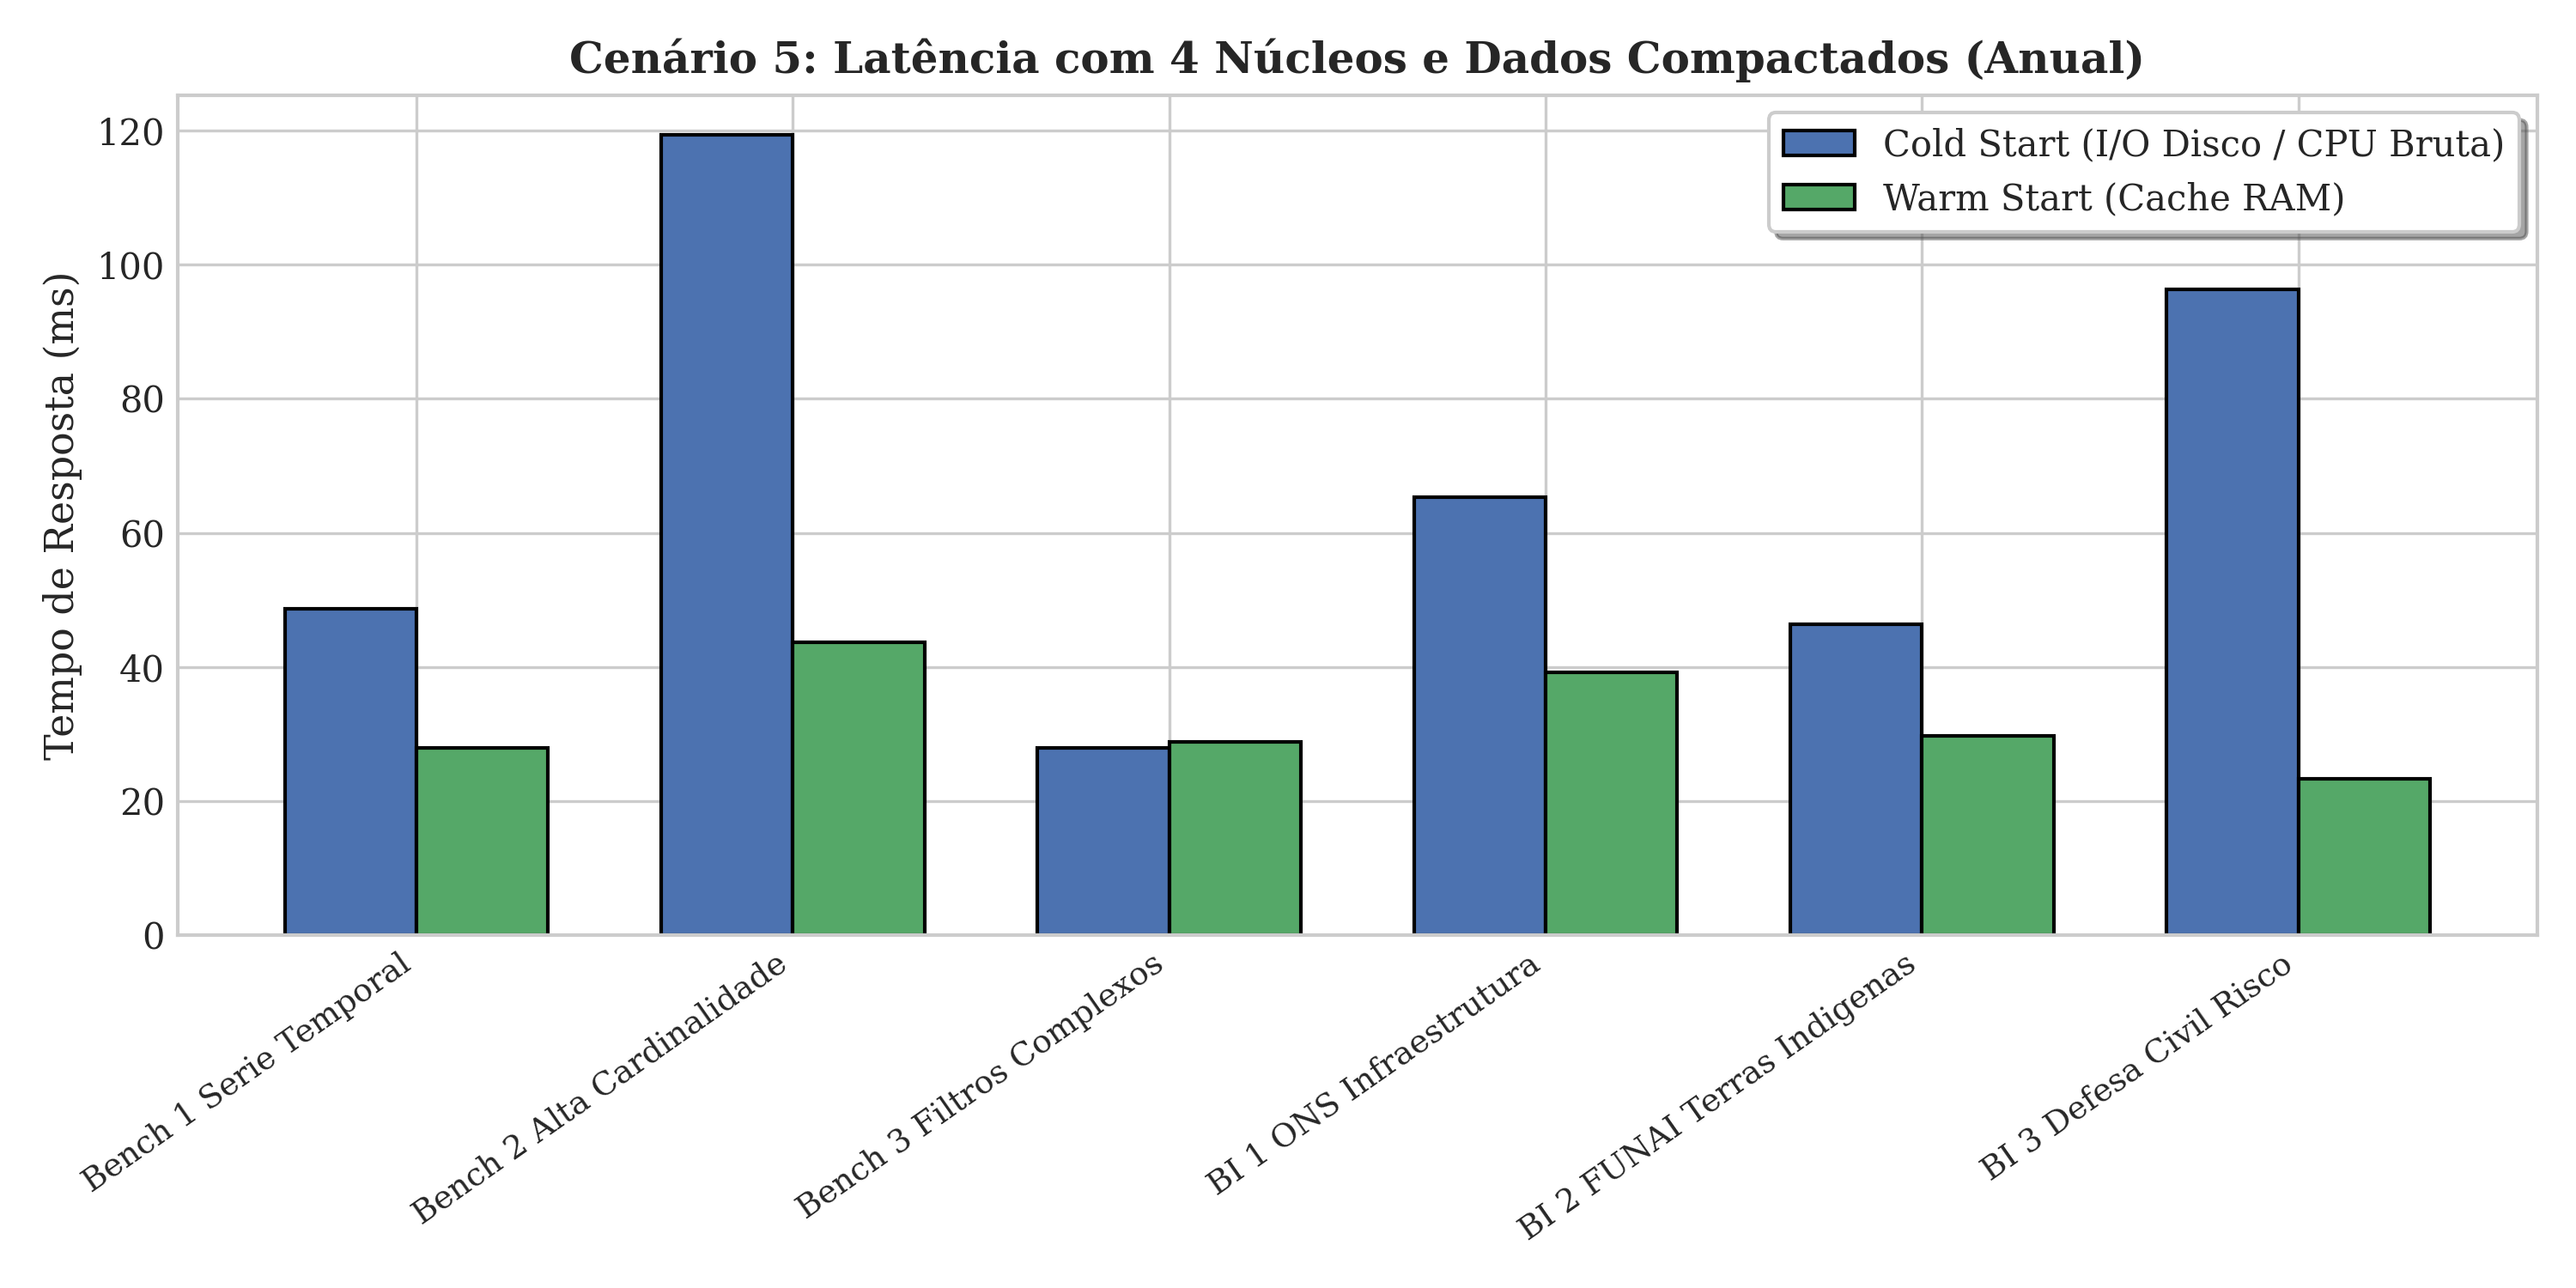
\includegraphics[width=0.9\textwidth]{fig_desemp_cenario5.png}
\caption{Comparativo geral evidenciando o limite assimptótico de latência.}
\end{figure}

Longe de ser uma falha estrutural, isto diagnostica uma exímia performance bruta. A consulta foi respondida com tanta velocidade pelos 4 núcleos interagindo com o disco mapeado que o custo logístico de interceptar, validar a \textit{query} e remontar as parciais via Memória RAM (\textit{Broker Cache}) tornou-se microscopicamente mais caro do que recalcular do zero.

\begin{figure}[H]
\centering
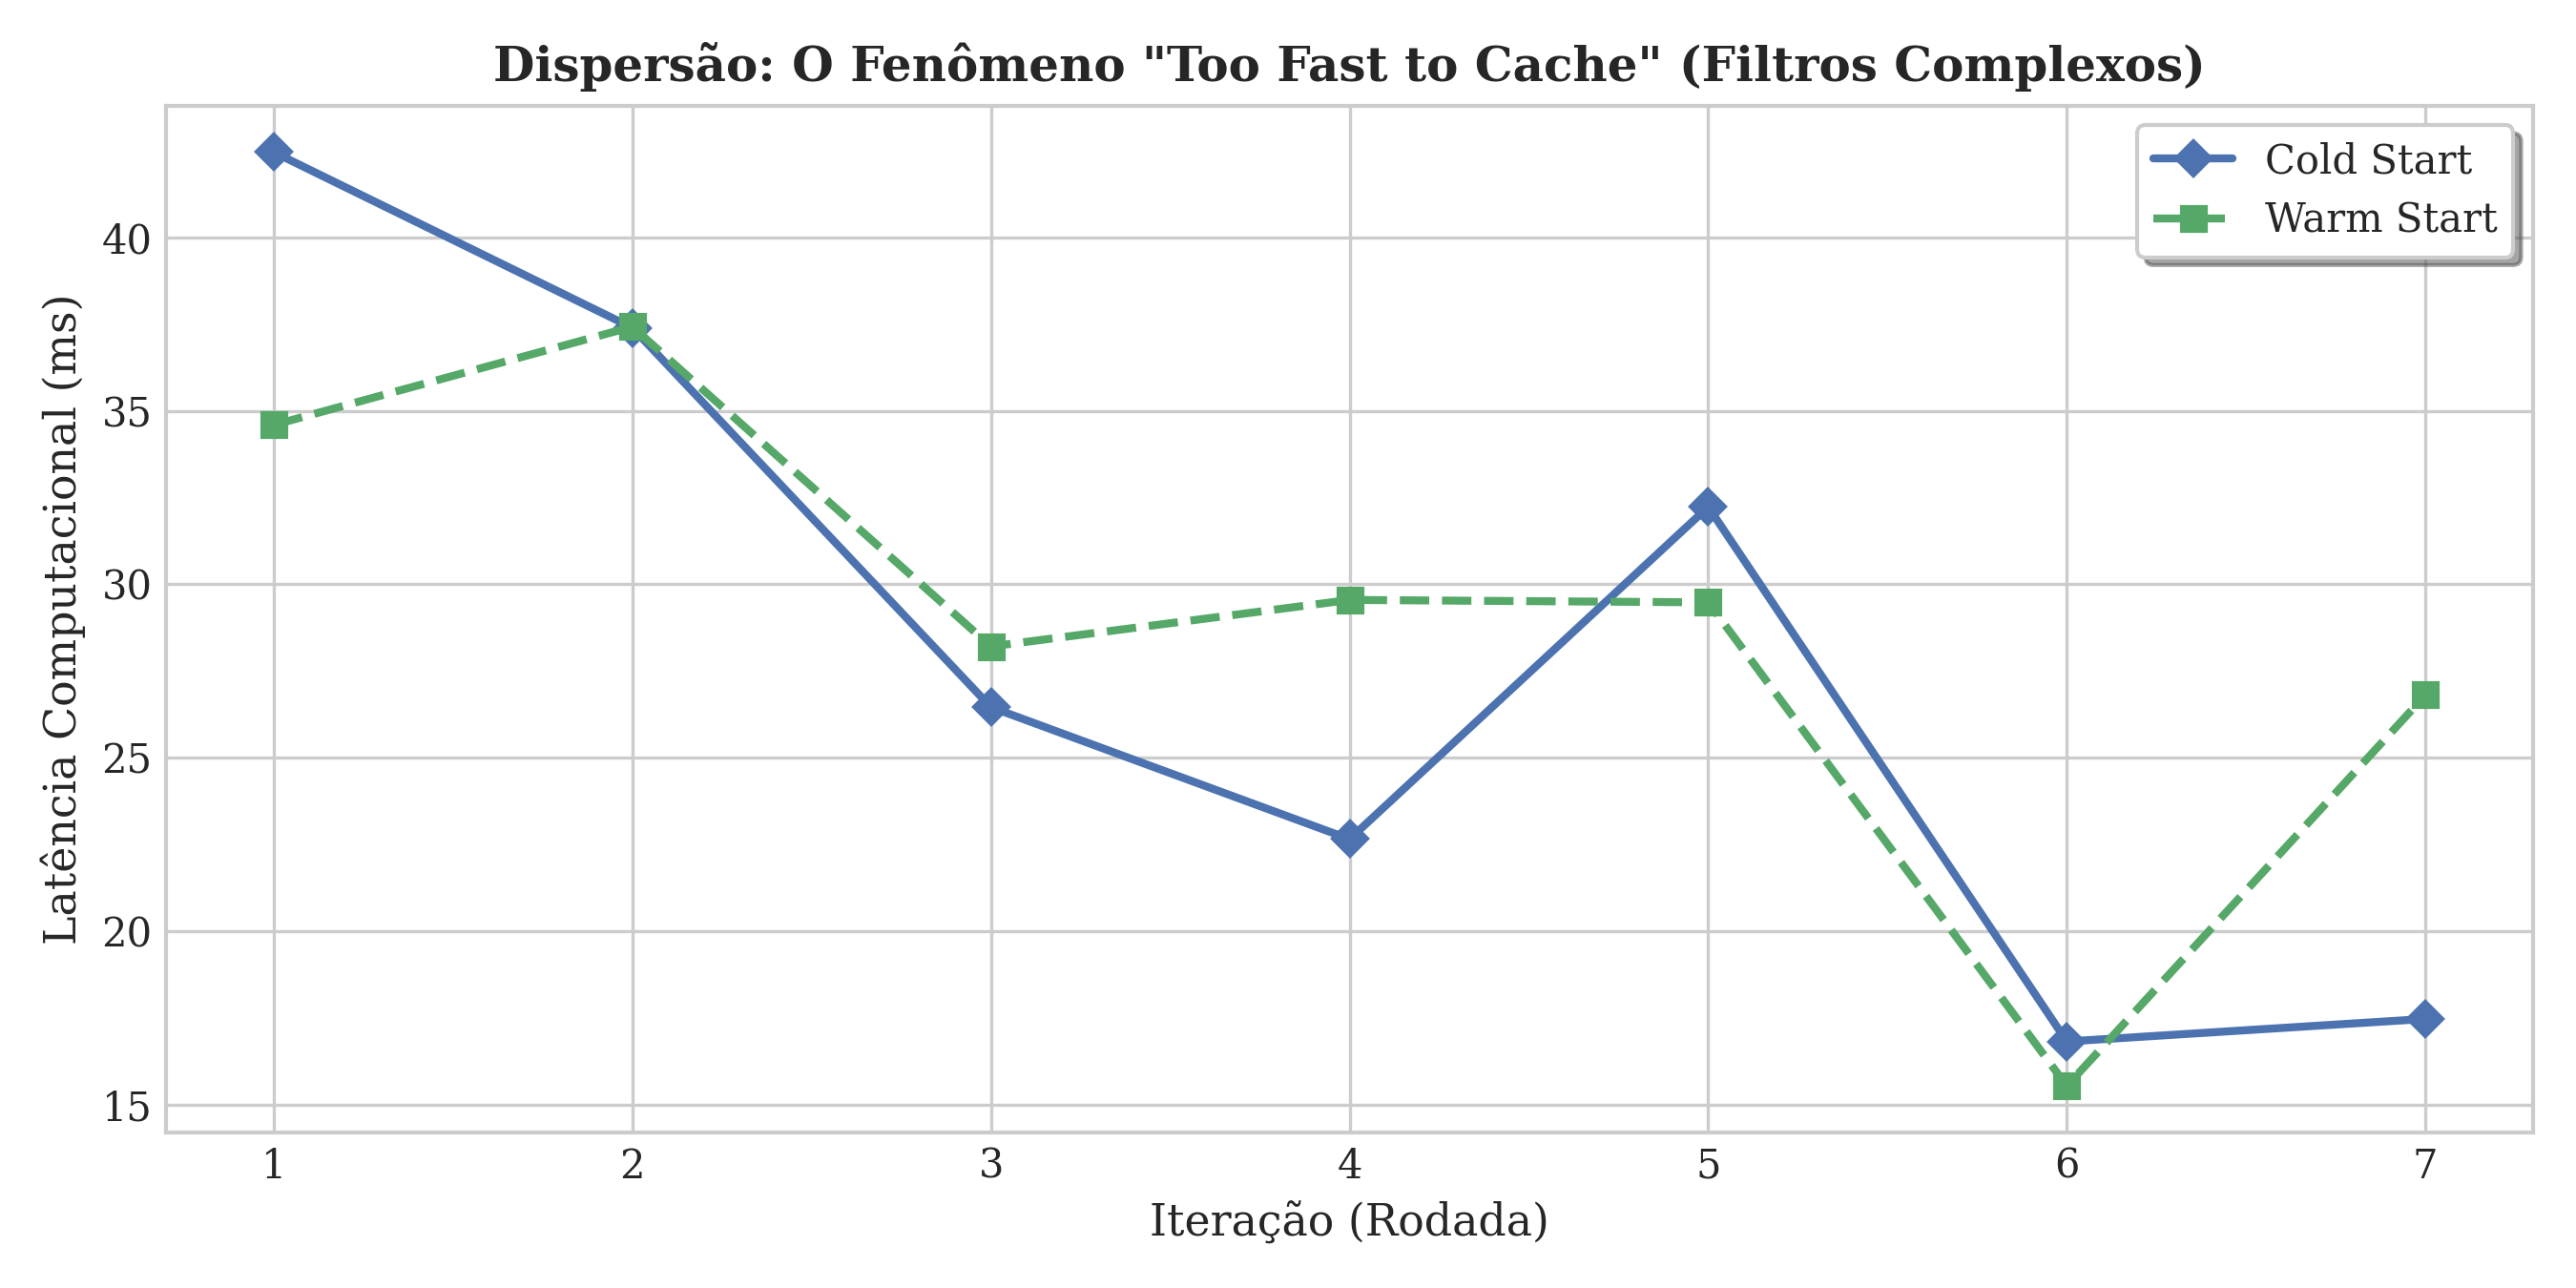
\includegraphics[width=0.8\textwidth]{fig_var_cenario5.png}
\caption{Dispersão da Latência ilustrando a colisão entre a velocidade do cache e do processador.}
\end{figure}

\section*{3. Conclusão da Intersecção de Camadas}
O Cenário 5 sela uma importante conclusão empírica: a infraestrutura (\textit{Hardware}) só extrai seu pleno potencial quando a camada de dados (\textit{DataOps}) está salutar. Ao atingirmos a faixa dos 20$\sim$100 ms generalizados, o Apache Druid atinge seu limite fisiológico imposto por restrições de rede e serialização (JSON), configurando um estado de \textit{Real-Time Analytics} irretocável. A etapa final testará 6 núcleos para avaliar se há algum residual a ser extraído do topo da curva assimptótica.

\end{document}
